
\subsection{State Design Pattern}


	\defn{State Design}{is one of the behavioural design patterns, which is used when an \ita{Object} changes its beahaviour based on its state}

	\rem{the object will appear to change its class}

	\par{Objects with a great number of states can become complex and hard to modify quite quickly. The naive way to implement states is to have a constant for each state and then implement a method for each state transition, which violates the \ita{open-close principle}. The key idea in this pattern is to introduce instead an abstract class to represent the behaviour which is common to all states, and represent those sates as subclasses of that interface}

	\rem{see refactoring example \texttt{gumball_machine.java}}


	\subsubection{Applicability}

		\par{The SDp is applicable when:}

		\begin{itemize}
			\item{an object's behaviour depends on its state, and its run-time behaviour must be changed according to that state}

			\item{operations have large, multipart conditional statements that depend on the object's state. The conditionalbranches can then be abstracted away and treated as objects in their own right}
		\end{itemize}

	\subsubsection{Structure}

		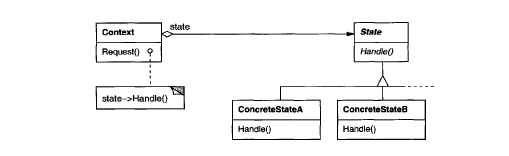
\includegraphics{pattern_state}
		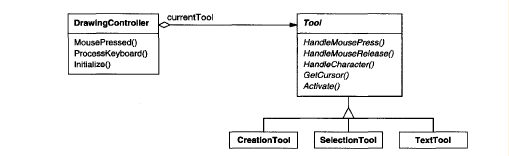
\includegraphics{pattern_state2}

	\subsection{Summary}

		\begin{itemize}
			\item the pattern encapsulates state into separate classes
			\item the context class delegates requests to the current state interface
			\item with each request the state may change
			\item composition is favoured over inheritance
			\item it abides by the \ita{open-closed principle} by allowing a class to remain open for extension, while being closed for modification
		\end{itemize}

